\documentclass[11pt]{beamer}
\beamertemplatenavigationsymbolsempty
\usetheme{Penn} 

\logo{}
\newcommand{\TODO}[1]{{\color{red}#1}}

\usepackage{epsfig, amsfonts, amsbsy, amsmath}
\usepackage{color}
\usepackage{amsmath}
\usepackage{amssymb}
\usepackage{scrextend}
\usepackage{float}
\usepackage{booktabs}
\usepackage{color}
\usepackage{graphicx}
\usepackage{cleveref}
\usepackage{relsize}
\usepackage{xspace} 
\usepackage{caption}
\usepackage{subcaption}
\usepackage{url}
\usepackage{natbib}
\usepackage[T1]{fontenc}
\usepackage[utf8]{inputenc}
\usepackage{multirow}
\usepackage{xcolor}
\usepackage{bbm}

% Copyright 2007 by Till Tantau
%
% This file may be distributed and/or modified
%
% 1. under the LaTeX Project Public License and/or
% 2. under the GNU Public License.
%
% See the file doc/licenses/LICENSE for more details.

\ProvidesPackageRCS $Header: /cvsroot/latex-beamer/latex-beamer/themes/color/beamercolorthemepenn.sty,v 1.4 2007/01/28 20:48:24 tantau Exp $

\definecolor{pennred}{cmyk}{0.75, 0.4, 1, 0.4}
\definecolor{pennblue}{cmyk}{1,0.7,0,0.30}



\mode<presentation>

\setbeamercolor*{palette primary}{use=structure,fg=white,bg= pennblue}
\setbeamercolor*{palette secondary}{use=structure,fg=white,bg= pennblue}
\setbeamercolor*{palette tertiary}{use=structure,fg=white,bg= pennblue}
\setbeamercolor*{palette quaternary}{fg=white,bg= pennblue}

\setbeamercolor*{sidebar}{use=structure,bg= pennblue}
  
\setbeamercolor*{palette sidebar primary}{use=structure,fg=structure.fg!10}
\setbeamercolor*{palette sidebar secondary}{fg=white}
\setbeamercolor*{palette sidebar tertiary}{use=structure,fg=structure.fg!50}
\setbeamercolor*{palette sidebar quaternary}{fg=white}

\setbeamercolor*{titlelike}{parent=palette primary}

\setbeamercolor*{separation line}{}
\setbeamercolor*{fine separation line}{}

\setbeamercolor{itemize item}{fg=pennblue}
\setbeamercolor{itemize subitem}{fg=pennblue}
\setbeamercolor{itemize subsubitem}{fg=pennblue}
\setbeamercolor{enumerate item}{fg=pennblue}
\setbeamercolor{enumerate subitem}{fg=pennblue}
\setbeamercolor{enumerate subsubitem}{fg=pennblue}
\setbeamercolor{description item}{fg=pennblue}


\mode
<all>

 \setbeamercovered{invisible}

\begin{document}

\author[]{\begin{tabular}{c} 
\\ \textbf{Team:} \\
{\small Martin Blapp}\\
{\small Doruk Çetin}\\
{\small Bernhard Kratzwald}\\
%{\small ... (order names alphabetically)}
\end{tabular}}

\date{Spring 2019}

\title{Combining Human and Machine Decisions}

\frame{
\begin{center}
{\small Fairness, Explainability, and Accountability for ML}
\end{center}
\titlepage}

\begin{frame}{Why combine human and machine decisions?}
\begin{itemize}
	\setlength\itemsep{1em}
	\item Decision problems that need human involvement:
	\begin{itemize}
	\item Jail-or-release
	\item Stop-and-frisk
	\item Accept-or-reject 
	\end{itemize}
	\item Human decision makers can profit from machine decisions:
		\begin{itemize}
		\item Reduce the workload
		\item Increase accuracy
		\item Enlarge fairness
	\end{itemize}
\end{itemize}
\end{frame}

\begin{frame}{Human and machine decisions}
\begin{itemize}
	\item How do we combine human and machine decisions?
	\item How are humans influenced by machine predictions? 
\end{itemize}
\centering
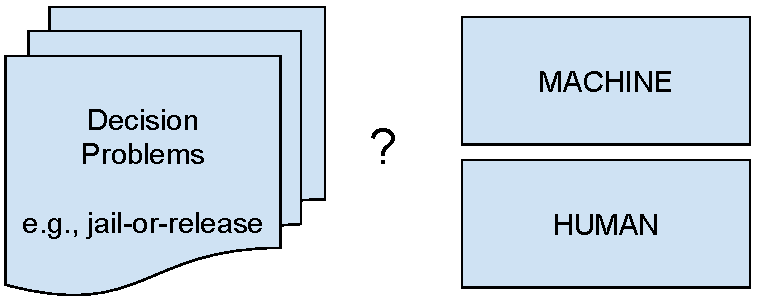
\includegraphics[width=0.5\textwidth]{Figures/problem_statement.pdf}
\end{frame}

\begin{frame}{Outline}
\begin{enumerate}
    \item Algorithm-in-the-loop analysis of fairness {\footnotesize [\cite{green2019disparate}]}\vspace{2pt}
    \item Matching decision problems to humans {\footnotesize [\cite{valera2018enhancing}]}\vspace{2pt}
    \item Learning to defer  {\footnotesize [\cite{madras2018predict}]}\vspace{2pt}
\end{enumerate}
\end{frame}

\begin{frame}{Algorithmic risk assessment}
\begin{figure}[t!]
    \centering
        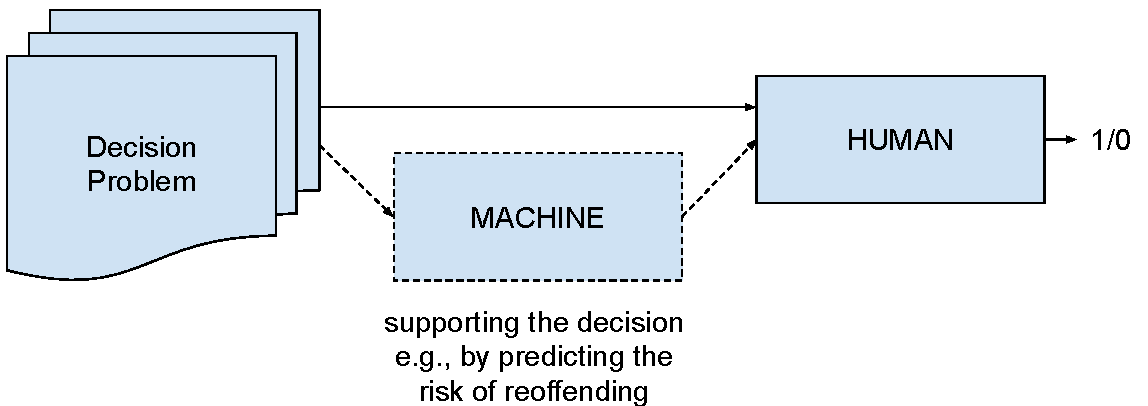
\includegraphics[width=0.8\textwidth]{Figures/human_decision.pdf}
\end{figure}
%\begin{itemize}
%\setlength\itemsep{5pt}%
%\item
+\quad Human makes the final decision
%\item 
+\quad Clear responsibility\vspace{4pt}
%\item 
--\quad What about fairness?
%\item
--\quad How is the human influenced by the machine prediction?
%\end{itemize}
\end{frame}

\begin{frame}{How are humans influenced by algorithmic risk assessments?}
\begin{itemize}
	\item Experiment on 500 pre-trial cases with known ground truth $y$
	\item Treatment group w/ algorithmic assessment ($N=6250$)
	\item Control group w/o algorithmic assessment ($N=7600$)
	%\item Entry and exit survey 
\end{itemize}
\begin{figure}[t!]
	\centering
	\footnotesize
	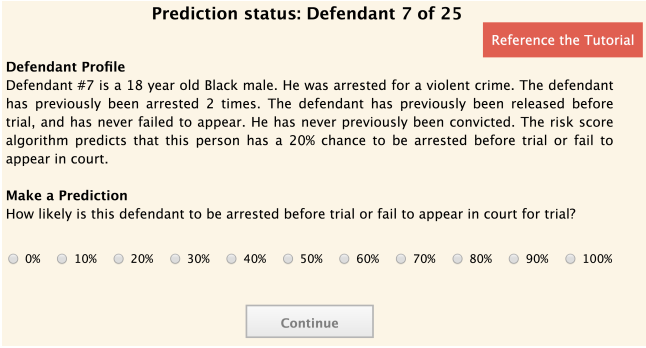
\includegraphics[width=0.7\textwidth]{Figures/experimentscreen.png}
	\caption{Amazon Turk experiment by \cite{green2019disparate}}
\end{figure}
\end{frame}

\begin{frame}{Performance under risk assessment}
\begin{table}[]
	\begin{tabular}{@{}lll}
		\toprule
		& \textbf{Control} & \textbf{Treatment} \\ \midrule
		Average reward      & 0,756            & 0,786               \\ \midrule
		False positive rate & 17.7\%           & 14.8\%              \\ \bottomrule
	\end{tabular}
\end{table}
\begin{itemize}
	\item Participants in the treatment group earned a 4.0\% larger average
	reward and a 16.4\% lower false positive rate than participants in the
	control group (both with $p < 10^{-5}$)
\end{itemize}
\end{frame}

\begin{frame}{Performance under risk assessment}
\begin{table}[]
	\begin{tabular}{@{}llll}
		\toprule
		& \textbf{Control} & \textbf{Treatment} &\textbf{Risk assessment} \\ \midrule
		Average reward      & 0,756            & 0,786 & 0.807               \\ \midrule
		False positive rate & 17.7\%           & 14.8\% & 10.1\%             \\ \bottomrule
	\end{tabular}
\end{table}
\begin{itemize}
	\item  Despite being presented with the risk assessment’s predictions, the treatment group achieved
	a 2.6\% lower average reward and a 46.5\% higher false positive rate
	than the risk assessment (both with $p < 10^{-8}$)
	\item  Only 23.7\% of participants in the treatment group earned a higher average reward than
	the risk assessment over the course of their trial
\end{itemize}
\end{frame}

\begin{frame}{Self evaluation of participants}
\begin{itemize}
	%\item Exit survey (confidence, accuracy of assessment, influence, fairness)
	\item The more confidence participants expressed in their predictions, the less well they actually performed ($p=0.0186$)
	\item No significant relationship between the participant's evaluation of the risk assessments accuracy and actual performance
	\item No significant relationship between actual and perceived fairness
	\item Participants could generally discern how strongly they were influenced by the risk assessment
\end{itemize}
\end{frame}

\begin{frame}{Influence of risk scores on defendants}
\begin{itemize}
\item When risk score was lower than the average prediction in control group ($r < c$):
\begin{itemize}
	\item Risk assessment's influence similar regardless of the race
\end{itemize}
\vspace{2pt}
\item When risk score was higher than the average prediction in control group ($r > c$):
\begin{itemize}
	\item 25.9\% stronger average influence on predictions about black defendants than on predictions about white defendants
	\item Risk assessment leads to larger increase in risk for black defendants
\end{itemize}
\end{itemize}
\end{frame}

\begin{frame}{Influence of risk scores on defendants}
\begin{figure}[t!]
	\centering
	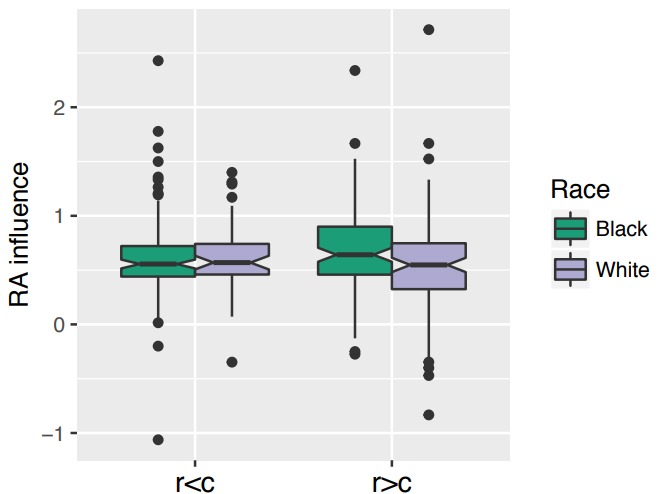
\includegraphics[width=0.8\textwidth]{Figures/influence_of_risk_score.png}
\end{figure}
\end{frame}

\begin{frame}{Limitations and Discussion}
\begin{itemize}
	\item Amazon Mechanical Turk and no actual judges
	\item Only textual description, no face-to-face \vspace{2pt}
	
	\item Maybe accuracy is not the metric we should optimize?
	\item Maybe risk assessment is not the optimal pattern? 
\end{itemize}
\end{frame}

\begin{frame}{Alternative pattern: Problem matching}
\begin{figure}[t!]
	\centering
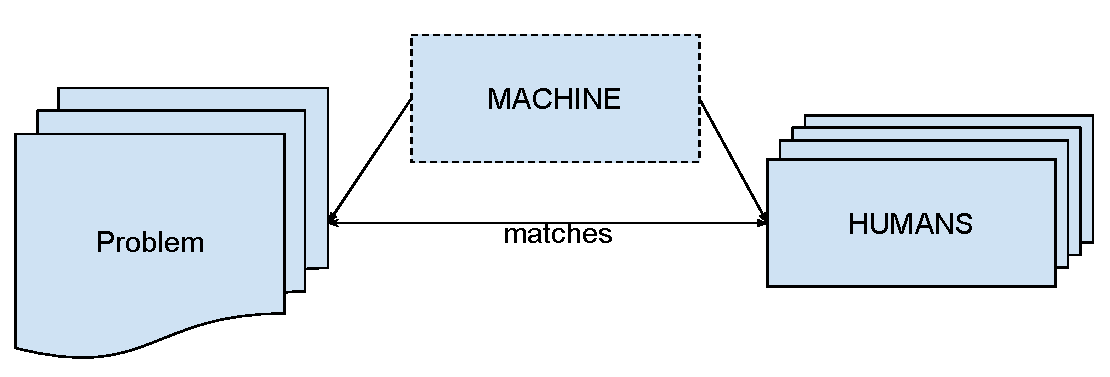
\includegraphics[width=0.8\textwidth]{Figures/matching.pdf}
\end{figure}
\end{frame}

\begin{frame}{Problem Definition}
\begin{figure}[t!]
\centering
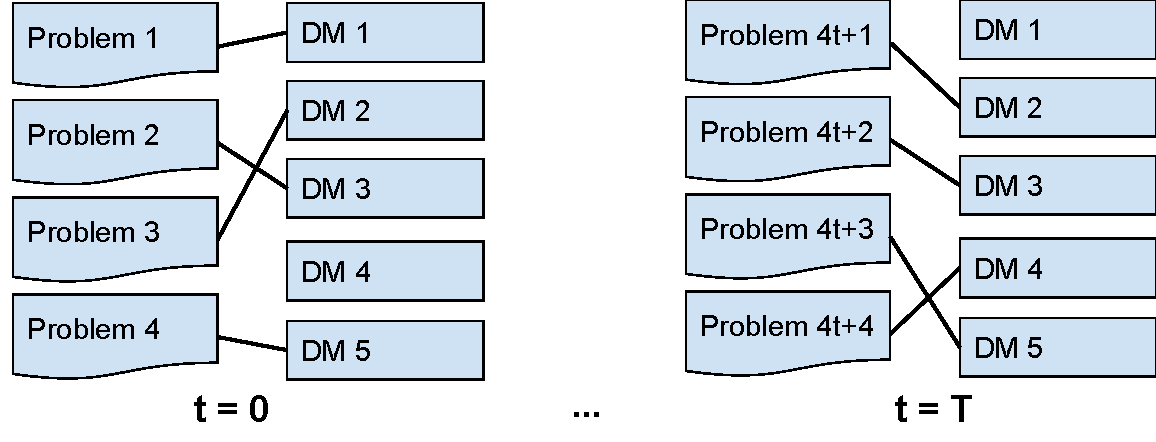
\includegraphics[width=0.7\textwidth]{Figures/matching_unfolded.pdf}
\end{figure}
each decision:
\begin{equation*}
\begin{gathered}
d_j(X_i,S_i)\rightarrow Y, \\
\text{where } X_i \in \mathbb{R}^d,  S_i \in \{0,1\}, Y_i \in \{0,1\}
\end{gathered}
\end{equation*}
\begin{center}
\text{we assume } $P(Y_i|X_i,S_i)$ known to decision makers, but each decision maker has own thresholds $\theta_{j,s}$
$
d_j(X_i,S_i) = 
\begin{cases}
1, & {\text{if } P(Y_i=1|X_i,S_i)\ge \theta_{j,S_i}} \\
0, & \text{otherwise}
\end{cases}
$
\end{center}
\end{frame}

\begin{frame}{Metrics}
We measure
\begin{itemize}
\item Utility
$$u(d,c)=\sum_{i\in \{decisions\}} Y_id(X_i,S_i)-cd(X_i,S_i)$$
\item Fairness Constraints \newline
$\Rightarrow$ Disparate Impact 
$$b_{s}= \mathbb{E} [1-d(X,S=s)]$$
$$DI=|b_{s=1}-b_{s=0}|\le \alpha$$
\end{itemize}
{\footnotesize See also [\cite{corbett2017algorithmic}]}
\end{frame}

\begin{frame}{Matching with known tresholds}
\begin{itemize}
\item Simple Case: Assume we know how humans decide, \newline$\theta_{j,s}$ are known
$\Rightarrow$ maximum weighted bipartite matching
$
w_{ji} = 
\begin{cases}
P(Y_i=1|X_i,S_i)-c, & \text{if } P(Y_i=1|X_i,S_i)\ge \theta_{j,S_i} \\
0, & \text{otherwise} \\
\end{cases}
$
\end{itemize}
\end{frame}

\begin{frame}{Matching with unknown thresholds}
\begin{itemize}
\item If human thresholds are unknown
\begin{itemize}
\normalsize
\setlength\itemsep{0.5em}
\item[--] initialize with prior $\theta_j(0) \sim Beta(\alpha ,\beta)$
\item[--] for each new round
$\theta_j(t+1) \sim p(\theta_j(t)|D(t))$
\item[--] maximum weighted bipartite matching
\end{itemize}
\end{itemize}
\begin{itemize}
\item Regret:
\quad $R(T)=u^*(d,c)-u(d,c)$
\begin{itemize}
\item[--] expected regret shrinks in $O(\sqrt{T})$
\end{itemize}
\end{itemize}
\end{frame}

\begin{frame}{Fairness Constraints}
When enforcing fairness constraints
$$DI=|b_{s=1}-b_{s=0}|\le \alpha$$
matching must satisfy for each s:
$$ m_{S=s}(b_{S=s}^*-\alpha)\le \sum_{\forall (i,j), S=s}\mathbb{1} (w_{ji}= 0)$$
$$\sum_{\forall (i,j), S=s}\mathbb{1} (w_{ji}= 0) \le  m_{S=s}(b_{S=s}^*+\alpha)$$
\scriptsize{
\begin{center}
    where $j\in\{humans\},i\in\{problems\}, m_{S=s}:=$ \#decisions with sensitive attribute s
\end{center}
}
\normalsize
bounded color matching problem 
$\Rightarrow$ bi-criteria algorithm with $\frac{1}{2}$-approximation guarantee.
\end{frame}

\begin{frame}{Results}
\centering
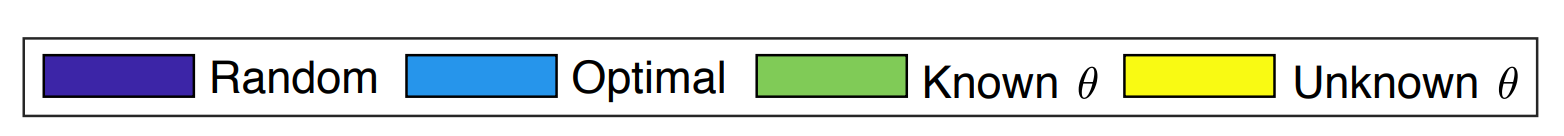
\includegraphics[width=0.8\textwidth]{Figures/paper2_results1.png}
\newline
\centering
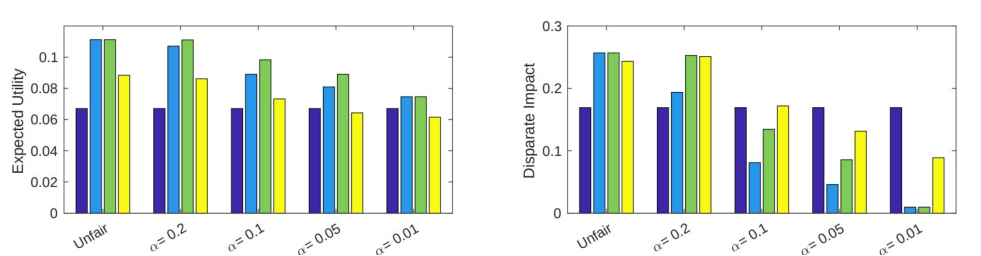
\includegraphics[width=1\textwidth]{Figures/paper2_results2.pdf}
\newline
\begin{itemize}
    \item wide range of $\theta_j$ beneficial
\end{itemize}
Limitations
\begin{itemize}
\item Assuming $P(Y|X,S)$ known to each DM
\item 1-Human to 1-Problem matching
\end{itemize}
\end{frame}

\begin{frame}{An alternative pattern: PASS option}
\begin{figure}[t!]
	\centering
	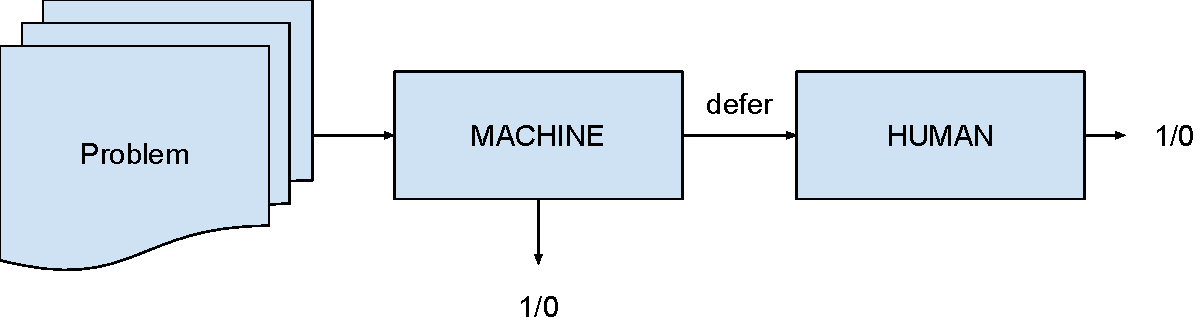
\includegraphics[width=0.8\textwidth]{Figures/defer.pdf}
\end{figure}
\end{frame}

\begin{frame}{Rejection learning}
$ \mathcal{L}_{reject}(Y,\hat{Y}_M, \hat{Y}_D, s) = 
- \mathlarger{\sum}\limits_i [(1-s_i) \ell(Y_i, \hat{Y}_{M,i}) + s_i \gamma_{reject}] $
\begin{itemize}
    \item $\hat{Y}_M $: decision of the machine learning model
    \item $\hat{Y}_D $: decision of the external decision maker
    \item $s$: gating variable (1 for rejections, 0 otherwise)
\end{itemize}
\vspace{60pt}
{\footnotesize Find more details here: [\cite{cortes2016learning}]}
\end{frame}

\begin{frame}{Learning to defer \citep{madras2018predict}}
\begin{multline}
  \mathcal{L}_{reject}(Y,\hat{Y}_M, \hat{Y}_D, s) =  \\ 
  - \mathlarger{\sum}\limits_i [(1-s_i) \ell(Y_i, \hat{Y}_{M,i}) + s_i \gamma_{reject}]
\end{multline}
\begin{multline}
  \mathcal{L}_{defer}(Y,\hat{Y}_M, \hat{Y}_D, s) =  \\ 
  - \mathlarger{\sum}\limits_i [(1-s_i) \ell(Y_i, \hat{Y}_{M,i}) + \textcolor{red}{s_i \ell(Y_i, \hat{Y}_{D,i})} + s_i \gamma_{defer}]
\end{multline}
\end{frame}

\begin{frame}{Setup}
\begin{itemize}
    \item COMPAS and Heritage Health datasets
    \item Equalized odds as fairness metric (Disparate impact as regularizer)
    \item ``Semi-synthetic data'': simulated DMs on real data
\end{itemize}
\end{frame}

\begin{frame}{Scenarios}
\begin{enumerate}[A)]
    \item High-accuracy DM: ignores fairness
    \item Highly-biased DM: strongly unfair
    \item Inconsistent DM: ignores fairness (noisy)
\end{enumerate}
In each scenario DM receives extra information (one feature) in training.
\end{frame}

\begin{frame}{Results: Scenarios A and B}
\begin{figure}[t!]
\centering
\begin{subfigure}[t]{0.5\textwidth}
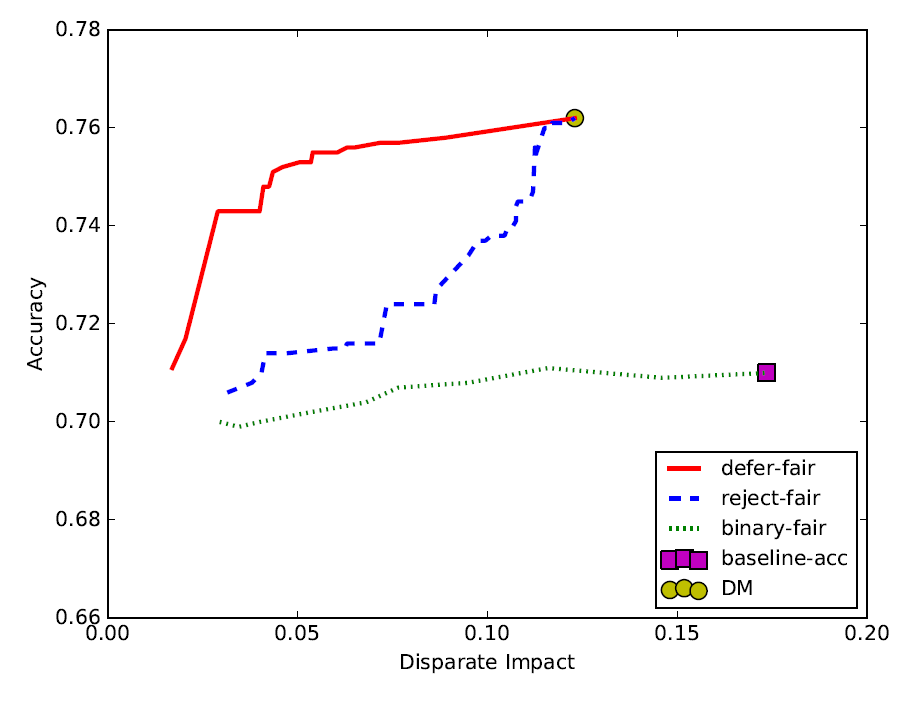
\includegraphics[width=\textwidth]{Figures/compasHighAcc.PNG}
\caption{High-accuracy DM}
\end{subfigure}%
\begin{subfigure}[t]{0.5\textwidth}
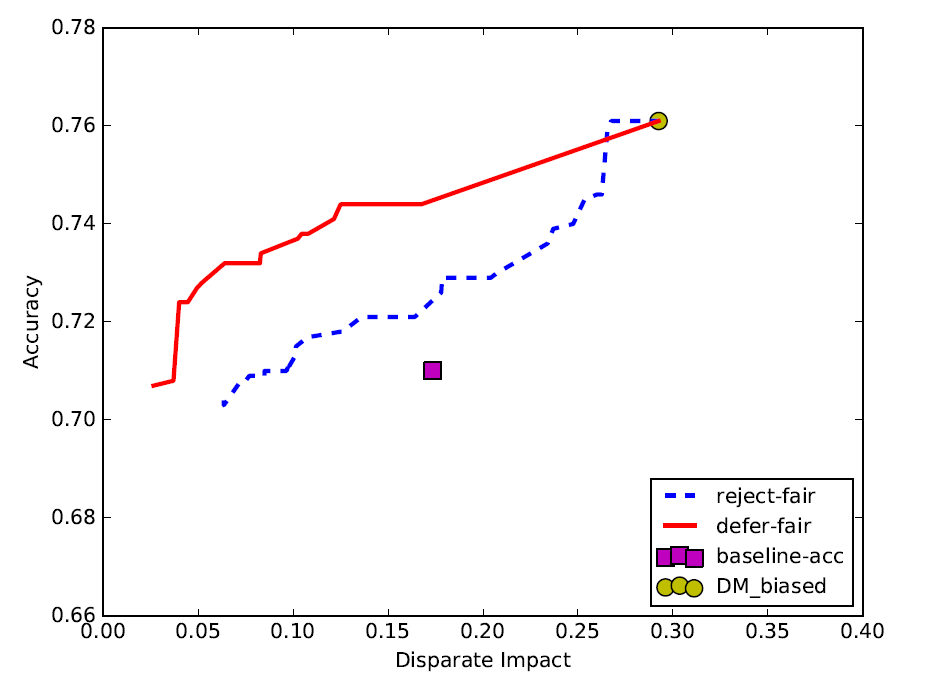
\includegraphics[width=\textwidth]{Figures/compasHighlyBiased.PNG}
\caption{Highly-biased DM}
\end{subfigure}
\end{figure}
\end{frame}

\begin{frame}{Results: Scenario C}
\begin{figure}[t!]
\centering
\begin{subfigure}[t]{0.4\textwidth}
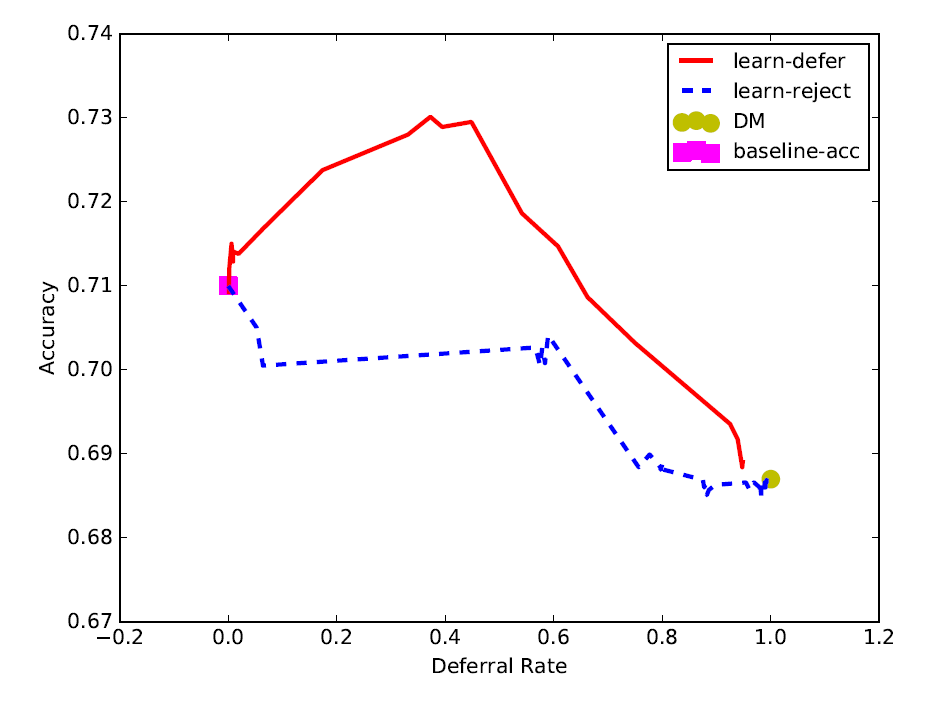
\includegraphics[width=\textwidth]{Figures/compasInconsistent.PNG}
\caption{Inconsistent DM}
\end{subfigure}%
\begin{subfigure}[t]{0.6\textwidth}
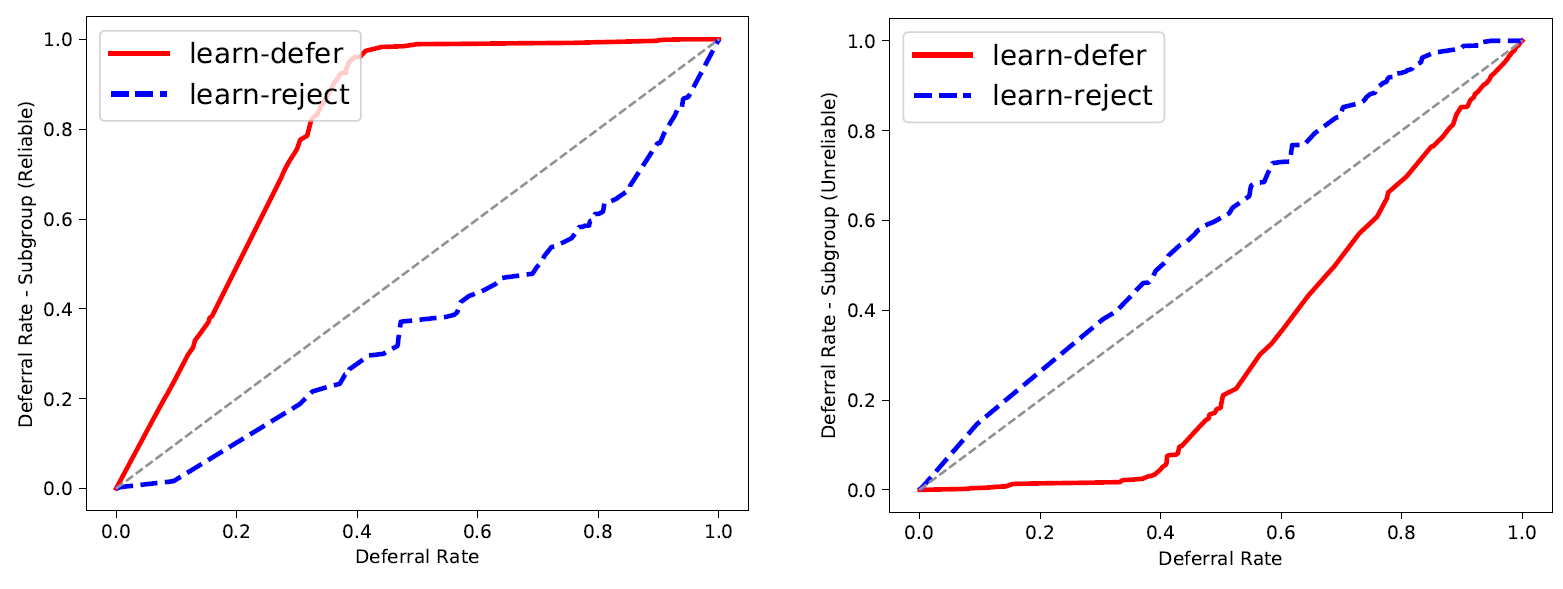
\includegraphics[width=\textwidth]{Figures/compasDeferralRatesC.PNG}
\caption{Deferral Rates}
\end{subfigure}
\end{figure}
\end{frame}

\begin{frame}{Why learning to defer?}
\begin{itemize}
    \item Adaptive rejection
    \item Considering the model impact
    \item Predicting responsibly
\end{itemize}
\end{frame}

\begin{frame}{Conclusion}
\begin{itemize}
    \item Great potential lies in the cooperation
    \begin{itemize}
        \item \cite{polson2018aiq}
    \end{itemize}
    \item Many nuances and pitfalls
    \begin{itemize}
        \item \cite{hamilton2015adventures}
    \end{itemize}
    \item Increasing importance
\end{itemize}
\end{frame}

\begin{frame}{References}
\scriptsize
\bibliographystyle{apalike}
\bibliography{Bibliography}
\end{frame}

% ADDITIONAL SLIDES HERE
\begin{frame}{Hypothesis}
\begin{itemize}
	\item \textbf{H1 (Performance): }Participants presented with a
	risk assessment will make predictions that are less accurate
	than the risk assessment’s.
	\item \textbf{H2 (Evaluation): }Participants will be unable to accurately evaluate their own and the algorithm’s performance.
	\item \textbf{H3 (Bias): }As they interact with the risk assessment, participants will be disproportionately likely to increase risk predictions about black defendants and to decrease risk predictions about white defendants.
\end{itemize}
\end{frame}

\begin{frame}{Evaluation}
\begin{itemize}
	\item Reward: $r = [1-(\text{prediction}-\text{outcome})^2]$\\
	\item Risk-score influence on defendant $j$: $$I_j = \frac{t_j - c_j}{r_j - c_j}$$
	\item Influence of risk assessment on participant $k$ is: $$I^k = \frac{1}{25}\sum^{25}_{i=1}\frac{p_i^k -c_i}{r_i-c_i}$$
\end{itemize}
{\footnotesize
$r_j \ldots$ prediction made by risk assessment 

$t_j \ldots$ avg. prediction of treatment group on defendant $j$ 

$c_j \ldots$ avg. prediction of control group on defendant $j$ 

$p_i^k \ldots$ prediction of participant $k$ on defendant $j$
}

\end{frame}

\begin{frame}{Learning to defer loss in detail}
\small
Final loss for learning to defer:
\begin{equation*}
\begin{split}
   \mathcal{L}_{defer}(Y,\hat{Y}_M, \hat{Y}_D, \pi; \theta)  
   & = \mathbb{E}_{s \sim Ber(\pi)} \mathcal{L}(Y,\hat{Y}_M, \hat{Y}_D, s; \theta) \\
   & = \sum\limits_i \mathbb{E}_{s \sim Ber(\pi)} [(1-s_i) \ell(Y_i, \hat{Y}_{M,i}; \theta) + s_i \ell(Y_i, \hat{Y}_{D,i})]
\end{split}
\end{equation*}

Loss function with fairness regularization:
\begin{equation*}
    \mathcal{L}_{defer}(Y,\hat{Y}_M, \hat{Y}_D, \pi; \theta) = \mathbb{E}_{s \sim Ber(\pi)} \mathcal{L}(Y,\hat{Y}_M, \hat{Y}_D, s; \theta) + \alpha_{fair} \mathcal{R}(Y, \hat{Y}_M, \hat{Y}_D, s)
\end{equation*}
The regularization term is a continuous relaxation of disparate impact (DI) as
\begin{equation*}
    \mathcal{R}(Y, \hat{Y}_M, \hat{Y}_D, s) = \frac{1}{2} (DI_{Y=0}(Y,A,\hat{Y}) + DI_{Y=1}(Y,A,\hat{Y}))
\end{equation*}
where
\scriptsize{
\begin{equation*}
    DI_{Y=i}(Y,A,\hat{Y}) = | \mathbb{E}_{\hat{Y}\sim Ber(p)} (\hat{Y}=1-Y|A=0,Y=i) - \mathbb{E}_{\hat{Y}\sim Ber(p)} (\hat{Y}=1-Y|A=1,Y=i) |
\end{equation*}
}
\end{frame}

\end{document}
